% MODELAGEM MATEMÁTICA PARA A OTIMIZAÇÃO DO EQUILÍBRIO SÓLIDO-LÍQUIDO------------------------------------------------------------------

\chapter{MODELAGEM MATEMÁTICA}
\label{chap:modelagem_matematica}

\section{Otimização}

O conceito de \textit{otimização} é uma forma de trazer uma solução satisfatória para problemas complexos que exigem a tomada de decisão ou alocação. \cite{Luenberger2016}

\section{Programação Não Linear}

Problemas reais são na grande maioria formulados por restrições, como a política de produção em uma grande empresa ou planejamento da agência governamental, são problemas de programação não linear com restrições.

Em geral o problema de programação é indicada por:
\begin{equation}
\begin{array}{rcccc}
\mbox{minimização} & f(x) & & & \\
\mbox{sujeita as condições} & h_{i}(x)&=&a_{i}, & i=1,2,\ldots,m \\
& g_ {j}(x)&\leq&b_j, & j=1,2,\ldots,p\\
& x\in S & & & \\
\end{array}
\end{equation}

Em que $x$ é um vetor n-dimensional $x=(x_{1},x_{2},\ldots,x_{n})$, $f_{i}$ e $h_i$ são funções reais das variáveis $x_{1},x_{2},\ldots,x_{n}$. A função $f$ é a \textit{função objetivo}, $g$, $h$ e o conjunto $S$ são as restrições do problema; com os parâmetros $a_i$ e $b_j$. \cite{Luenberger2016, Rocha2009a}

\section{Convexidade}

Os conceitos relacionados aos conjuntos \textit{convexos} são relevantes teoria da otimização, representada pela Figura \ref{fig:convexSet} na forma bidimensional, que por sua vez é essencial para um estudante de otimização ter conhecimento de suas propriedades mais fundamentais. \cite{Luenberger2016, Rocha2009a}

\begin{definicao}
	Dado um conjunto $C\subset E^{n}$ diz que é \textbf{convexo} se para qualquer $x_{1}, x_{2} \in C$ e para todo $\alpha\in\mathbb{R}$, tal que o ponto $\alpha x_{1}+(1-\alpha)x_{2}\in C$.
\end{definicao}

%\begin{comment}
\begin{figure}[H]
	\centering
	\subbottom[Convexo]{
		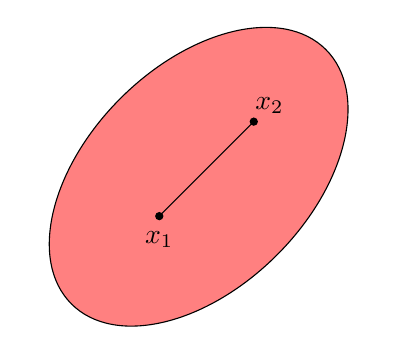
\begin{tikzpicture}
		\draw[rotate=-45,fill=red!50] (0,0) ellipse (40pt and 65pt);
		\draw (-0.5,-0.5) -- (0.7,0.7);
		\fill (-0.5,-0.5) circle[radius=1.5pt];
		\fill (0.7,0.7) circle[radius=1.5pt];
		\node at (-0.5,-0.8) {$x_1$};
		\node at (0.9,0.9) {$x_2$};
		\end{tikzpicture}}
	\hspace{2cm}
	\subbottom[Não Convexo]{
		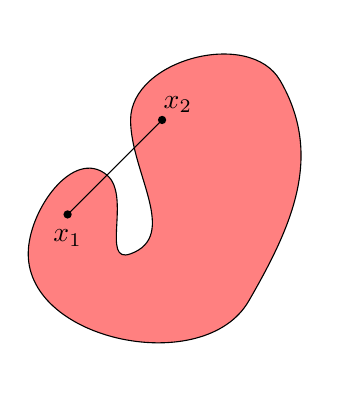
\begin{tikzpicture}
		\draw[fill=red!50] (0,0) to [out=140,in=90] (-1,-1)
		to [out=-90,in=240] (1.8,-1.6)
		to [out=60,in=-60] (2.2,1.2)
		to [out=120,in=90] (0.3,0.7)
		to [out=-90,in=20] (0.3,-1)
		to [out=200,in=-40] (0,0);
		\draw (-0.5,-0.5) -- (0.7,0.7);
		\fill (-0.5,-0.5) circle[radius=1.5pt];
		\fill (0.7,0.7) circle[radius=1.5pt];
		\node at (-0.5,-0.8) {$x_1$};
		\node at (0.9,0.9) {$x_2$};
		\end{tikzpicture}}
	\caption{Convexidade de conjuntos}
	\label{fig:convexSet}
\end{figure}

\section{\textit{Softwares} Utilizados}

Os \textit{softwares} utilizados para o desenvolvimento do trabalho, foram descritos nos subitens que seguem.

\subsection{\textit{Geogebra}}
Para a coleta de pares ordenados e organização das misturas binárias para fins de cálculos vamos utilizar o \textit{software} \textit{Geogebra}\footnote{Site do Geogebra \url{https://www.geogebra.org/}} é um \textit{software} de código aberto Figura \ref{fig:11}, oferecido para várias plataformas, com a finalidade didática e de pesquisa. 
\begin{figure}[H]
	\centering
	\includegraphics[width=0.9\linewidth 
	%,height=0.4\textheight
	]{dados/figuras/Geogebra_1.png}
	\caption[Site do Geogebra]{Site do Geogebra}
	\label{fig:11}
\end{figure}


\subsection{\textit{PyCharm} e \textit{R}}

Os \textit{software} \textit{PyCharm}\footnote{Site do \textit{PyCharm} \url{https://www.jetbrains.com/pt-br/pycharm/}} (FIGURA \ref{fig:11}) possui licença gratuita com restrições, disponíveis para as principais plataformas e, conjuntamente com a utilização da biblioteca \textit{R}\footnote{A base de dados para implementação de modelos estatísticos disponível no site \url{https://cran.r-project.org/}} (FIGURA \ref{fig:11}), se apresentam como uma base para implementação de algoritmos e modelos estatísticos. 



\subsection{Editor de texto \LaTeXe}

\LaTeXe  é o \textit{software} de código aberto de alta qualidade afim de produzir impressões profissionais e arquivos PDF, cuja base de dados \textit{TexLive}\footnote{Se encontra no site \url{http://tug.org/texlive/}} para plataformas Linux e macOS, organizada por \textit{TeX User Group} instituição sem fins lucrativos fundada em 1980, composto por \TeX\ \ criado por Donald Knuth e a mais conhecida ou difundida \textit{MikTex}\footnote{Se encontra no site \url{https://miktex.org/}} para todas as plataforma. A interface gráfica foi utilizado o \textit{TeXstudio}\footnote{Se encontra no site \url{https://www.texstudio.org/}} e \textit{Overleaf}\footnote{Se encontra no site \url{https://pt.sharelatex.com/}} uma ferramenta online para trabalhos colaborativos com o sistema de versionamento podendo ver quais são as modificações feitas por cada um colaborador. A a principal finalidade do \LaTeX é trazer uma tipografia de alta qualidade com o intuito trazer uma leitura mais agradável visualmente, com a biblioteca \textit{amsmath} para escrever fórmulas matemática, \textit{tikz} para criar desenhos vetoriais como os desenhos Figura\ref{fig:convexSet} e Figura\ref{fig:11}, \textit{chemformula} para fórmulas químicas, colabora com citação, facilita indexação de elementos e entre outras funcionalidades. \cite{latexchemformula,latexabntex2,latextikz,tex}


